\documentclass[tikz,border=5pt]{standalone}
\usepackage[UTF8]{ctex}
\usepackage{amsmath,amssymb}
\usetikzlibrary{arrows.meta,calc,angles,quotes,decorations.pathmorphing}
\definecolor{ink}{HTML}{243447}\definecolor{blue}{HTML}{2765A2}
\definecolor{green}{HTML}{3F7D5B}\definecolor{red}{HTML}{B74739}
\tikzset{body/.style={draw=ink,thick},vec/.style={draw=blue,thick,-{Latex}},guide/.style={gray!65,dashed},dim/.style={ink,{Latex}-{Latex}},line cap=round,line join=round}
\begin{document}
\begin{tikzpicture}
\coordinate(A)at(0,3.464);\coordinate(B)at(-2,0);\coordinate(C)at(2,0);
\draw[body](A)--(B)--(C)--cycle;
\foreach \p/\n/\lab in {A/1/above,B/2/below left,C/3/below right}{
\fill[blue](\p)circle(.11);\node[\lab]at(\p){第$\n$人：$m,\mu_\n$};}
\node at(0,-1){俯视图；三根轻绳分别沿三边连接};
\end{tikzpicture}
\begin{tikzpicture}
\coordinate(A)at(0,3.464);\coordinate(B)at(-2,0);\coordinate(C)at(2,0);
\draw[guide](A)--(B)--(C)--cycle;
\foreach \p in {A,B,C}{\fill[ink](\p)circle(.06);}
\draw[vec](A)--($(A)!.31!(B)$)node[midway,left]{$T_{12}$};
\draw[vec](A)--($(A)!.31!(C)$)node[midway,right]{$T_{13}$};
\draw[green,thick,-{Latex}](B)--($(B)!.31!(A)$)node[midway,left]{$T_{12}$};
\draw[green,thick,-{Latex}](B)--($(B)!.31!(C)$)node[midway,below]{$T_{23}$};
\draw[red,thick,-{Latex}](C)--($(C)!.31!(A)$)node[midway,right]{$T_{13}$};
\draw[red,thick,-{Latex}](C)--($(C)!.31!(B)$)node[midway,below]{$T_{23}$};
\draw[ink](A)++(-.3,-.52)arc(240:300:.6);
\node at(0,2.62){$60^\circ$};
\node[above]at(A){1};\node[below]at(B){2};\node[below]at(C){3};
\node at(0,-.9){地面摩擦抵消各顶点的张力合力};
\end{tikzpicture}
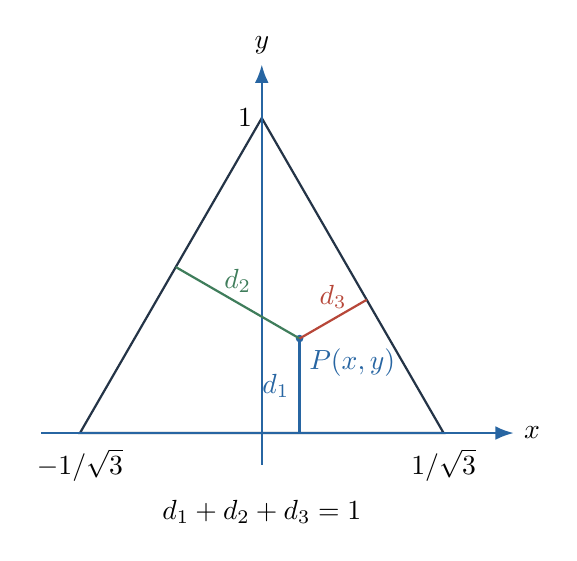
\begin{tikzpicture}[scale=4]
\draw[body](-.57735,0)--(0,1)--(.57735,0)--cycle;
\draw[vec](-.7,0)--(.8,0)node[right]{$x$};
\draw[vec](0,-.1)--(0,1.17)node[above]{$y$};
\coordinate(P)at(.12,.3);
\fill[blue](P)circle(.012)node[below right]{$P(x,y)$};
\draw[blue,thick](P)--(.12,0)node[midway,left]{$d_1$};
\draw[green,thick](P)--(-.2731,.5270)node[midway,above]{$d_2$};
\draw[red,thick](P)--(.33311,.42304)node[midway,above]{$d_3$};
\node[below]at(-.57735,-.02){$-1/\sqrt3$};\node[below]at(.57735,-.02){$1/\sqrt3$};
\node[left]at(0,1){$1$};
\node at(0,-.25){$d_1+d_2+d_3=1$};
\end{tikzpicture}
\begin{tikzpicture}[scale=5]
\fill[gray!9](-.57735,0)--(0,1)--(.57735,0)--cycle;
\foreach \angle/\col in {0/blue,120/green,240/red}{
\begin{scope}[rotate around={\angle:(0,.333333)}]
\fill[\col!14](-.288675,.5)--(0,1)--(.288675,.5)
--plot[domain=.288675:-.288675,samples=80]({\x},{-3+sqrt(12+3*\x*\x)})--cycle;
\draw[\col,thick,domain=-.288675:.288675,samples=80]plot({\x},{-3+sqrt(12+3*\x*\x)});
\end{scope}}
\draw[body](-.57735,0)--(0,1)--(.57735,0)--cycle;
\node[blue]at(0,.72){1安全};\node[green]at(-.32,.16){2安全};\node[red]at(.32,.16){3安全};
\node at(0,.34){无人安全};
\node at(0,-.16){边界弧为临界状态，不计入严格安全区};
\end{tikzpicture}
\end{document}
